\subsection{Non-Probabilistic Entropy}

\subsubsection{Fuzzy entropy description}
%==============================================================================
\label{sssec:desc}

De-Luca \& Termini fuzzy entropy algorithm \cite{DeLuca_Termini_1972} is considered to be the first to build upon Shannon entropy. Their implementation takes into account a set of data, along with their various membership degrees.


\begin{equation}
  \label{eq:de-luca}
  H_A = -K \displaystyle\sum_{i=1}^{n}{\{\mu_i\log(\mu_i) + (1 - \mu_i)\log(1 - \mu_i)\}}
\end{equation}

Al-sharhan et al's paper compiling several Fuzzy Entropy algorithms \cite{Al-Sharhan_Karray_Gueaieb_Basir_2001} contains a methodical,in-depth derivation of their algorithm, and has been instrumental in building my knowledge on the algorithm in question.

We will assume $-K$, the positive constant, is defined as $\frac{1}{n}$ as outlined in \cite{DeLuca_Termini_1972}.

%==============================================================================
\subsubsection{MATLAB implementation}
%==============================================================================

After some research into current implementations of Fuzzy Entropy algorithms in MATLAB, it was concluded the best approach would be to implement De-Luca \& Termini's algorithm from scratch. This entailed creating a membership class, which computes the grey-level membership of each pixel in the mean image (calculated from a set of input images).

This array of pixel memberships is fed into a `De Luca' function where it is iteratively passed into latter part of equation \ref{eq:de-luca} (after $\displaystyle\sum$). The output array is then summed and multiplied by $\frac{1}{n}$ as defined in Section \ref{sssec:desc}. The final mean pixel entropy is calculated by taking the image entropy and dividing by the number of pixels in the image.

This is all relatively straight forward to implement in MATLAB, as it is designed to run mathematical equations.


%==============================================================================
\subsubsection{Technical challenges}
%==============================================================================

The main technical challenge for this implementation is ensuring maximum optimisation to keep running times to a minimum. Leveraging MATLAB's own functions for the membership saves a lot of time and lines of code, however it's been important to check what they call from within. One membership function was redrawing the trapeziums every time it was called, significantly slowing down the process - reducing the amount of times the initial function was called helped reduced the run-time by over 60seconds.

Another technical challenge faced whilst implementing the De Luca \& Termini algorithm, isn't directly tied to the implementation of their specific equation, but more of my lack of experience in MATLAB, slowing down the programming rate. It has indeed been a steep learning curve, getting to grips with standard error messages, the debugger tool and knowing which `Toolboxes' are needed to run specific MATLAB functions.

Finally, as can be ascertained from Figure \ref{fig:mammo-results}, when writing the 4 seperate scans into 1 larger file, somewhere the images get rotated. This will be a reoccurring issue through the 3 Fuzzy entropy implementations, however as this is the first I will note it here. I think this is caused thanks to the swapping of the height and width values, however upon initial inspection of the file writing function, it is not clear as to which line is causing this issue. This issue has been marked low priority in the short term, due to all the scans being rotated in this fashion, and as such all have the same orientation. This means the congealing algorithm can work with no issues upon these images, the rotation is more merely an aesthetic issue.

%==============================================================================
\subsubsection{Results}
%==============================================================================

\begin{figure}[!ht]
  \centering
  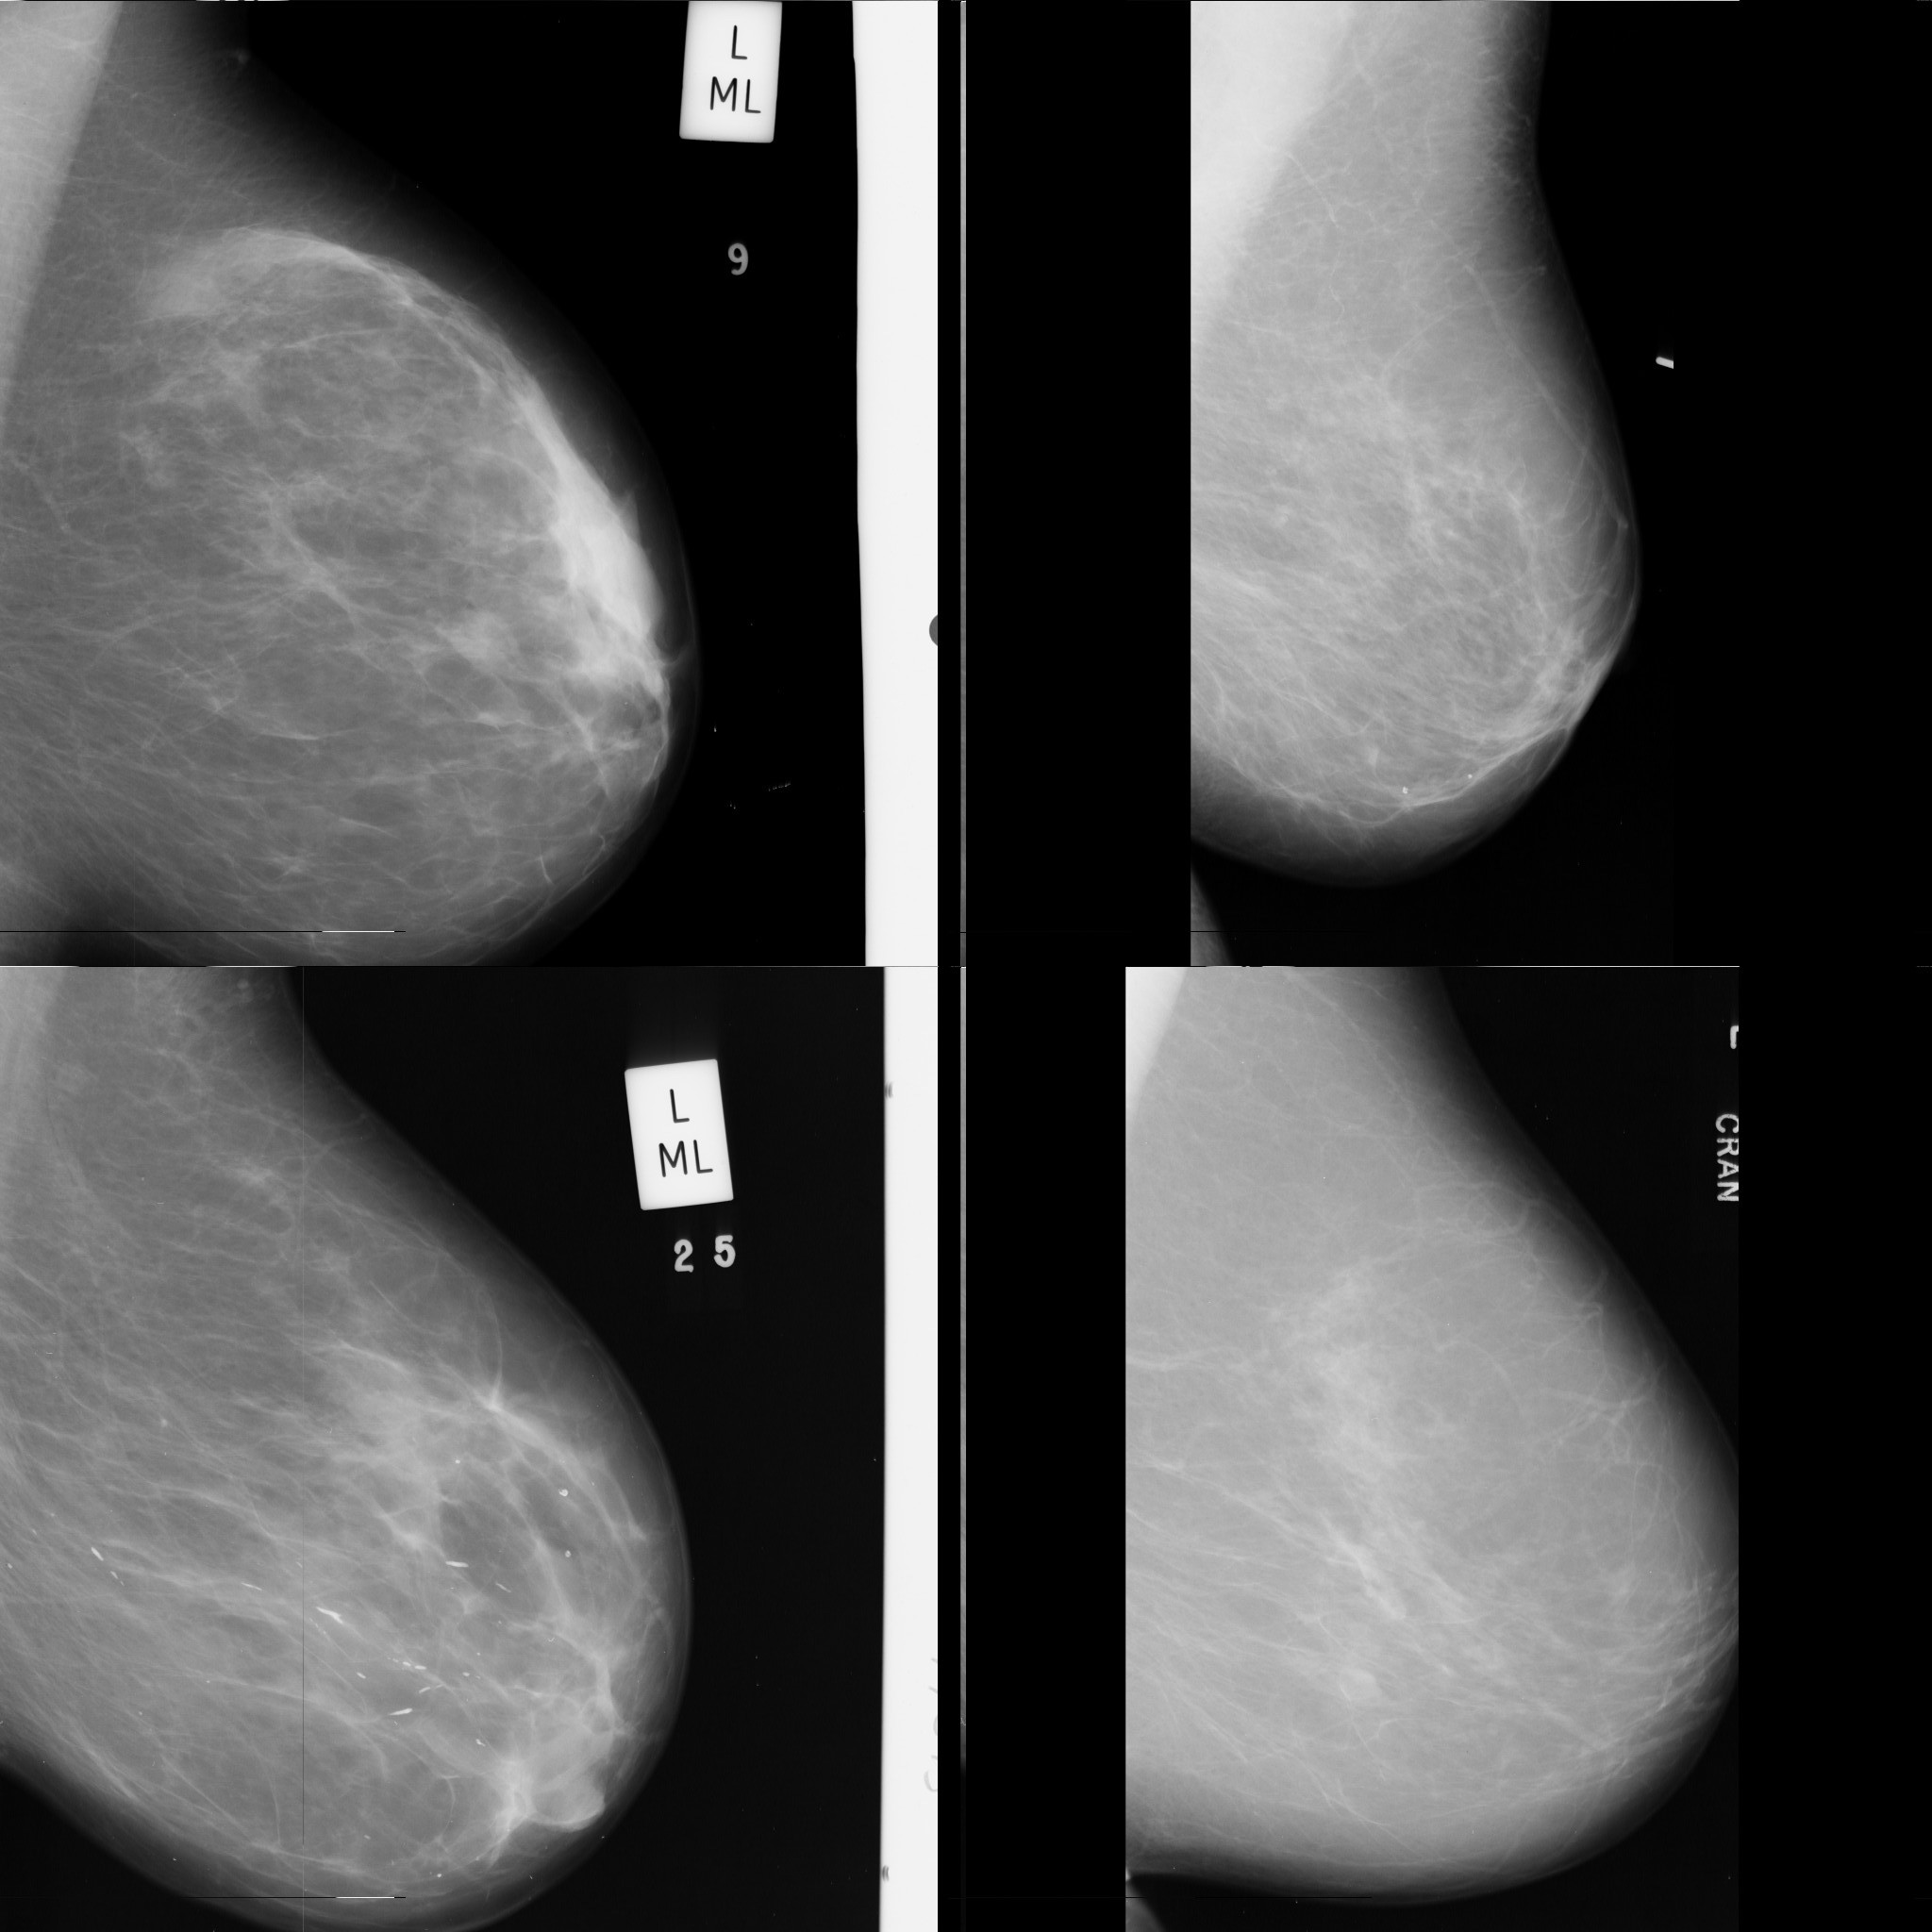
\includegraphics[width=0.4\textwidth]{Chapter2/non-prob-img/big_scan_1.jpg}
  \caption{4 input images of BI-RADS I classification}
  \label{fig:input}
\end{figure}

\begin{figure}[!ht]
    \centering
    \begin{subfigure}[b]{0.4\textwidth}
        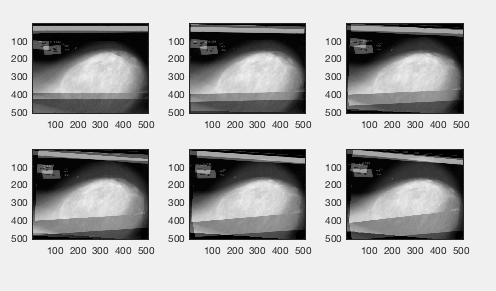
\includegraphics[width=\textwidth]{Chapter2/non-prob-img/iteration-mean.png}
        \caption{Mean image over each iteration}
        \label{fig:mean-imgs}
    \end{subfigure}
    ~ %add desired spacing between images, e. g. ~, \quad, \qquad, \hfill etc.
      %(or a blank line to force the subfigure onto a new line)
    \begin{subfigure}[b]{0.4\textwidth}
        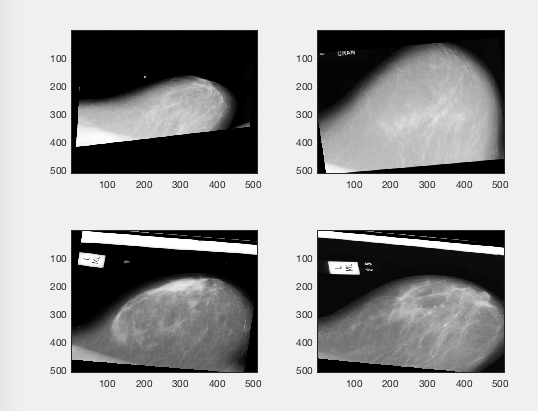
\includegraphics[width=\textwidth]{Chapter2/non-prob-img/adj-ser.png}
        \caption{Adjusted original input images}
        \label{fig:adj-ser}
    \end{subfigure}
    \caption{Output of 5 congealing iterations}\label{fig:mammo-results}
\end{figure}

\begin{figure}[!ht]
  \centering
  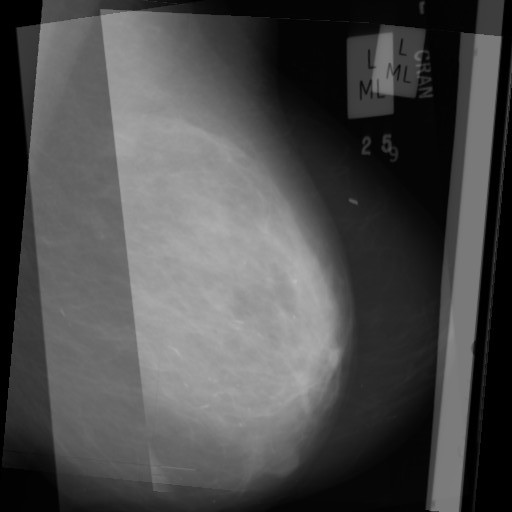
\includegraphics[width=0.4\textwidth]{Chapter2/non-prob-img/final_mean.jpg}
  \caption{Final mean image after 5 iterations (bottom-right most in Figure \ref{fig:mammo-results})}
  \label{fig:final-mean}
\end{figure}

\subsubsection{Entropy results}

  \begin{tabular}{ | l | r | }
    \hline
    \textbf{Iteration} & \textbf{Entropy} \\
    \hline
    1 & 0.050519 \\ \hline
    2 & 0.043925 \\ \hline
    3 & 0.035679 \\ \hline
    4 & 0.029035 \\ \hline
    5 & 0.026194 \\ \hline
  \end{tabular}

\subsubsection{Time to Run}

\begin{figure}[!ht]
  \centering
  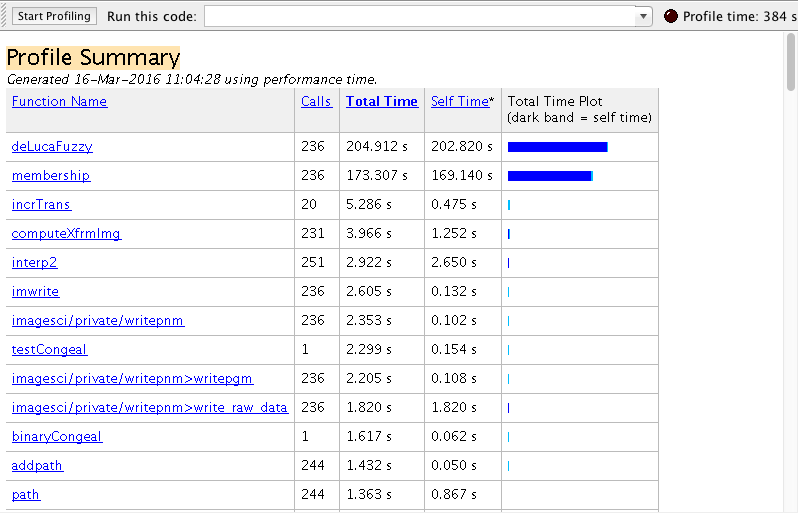
\includegraphics[width=0.8\textwidth]{Chapter2/non-prob-img/Run-time.png}
  \caption{Snapshot of run-time statistics}
  \label{fig:run-time}
\end{figure}
